\documentclass[conference]{IEEEtran}
\IEEEoverridecommandlockouts
% The preceding line is only needed to identify funding in the first footnote. If that is unneeded, please comment it out.
\usepackage{cite}
\usepackage{amsmath,amssymb,amsfonts}
\usepackage{algorithmic}
\usepackage{graphicx}
\usepackage{textcomp}
\usepackage{xcolor}
\def\BibTeX{{\rm B\kern-.05em{\sc i\kern-.025em b}\kern-.08em
		T\kern-.1667em\lower.7ex\hbox{E}\kern-.125emX}}
\begin{document}
	
	\title{Project Management Chatbot}
	
	\author{\IEEEauthorblockN{ Nahin Peñaranda}
		\IEEEauthorblockA{20231020032\\
			\textit{Systems Engineering } \\
			njpenarandam@udistrital.edu.co}
		\and
		\IEEEauthorblockN{Manuel Guerrero}
		\IEEEauthorblockA{20231020078\\
			\textit{Systems Engineering } \\
			mrguerreroc@udistrital.edu.co}
		
	}
	
	\maketitle
	
	\begin{abstract}
		This paper presents the development and system analysis of a chatbot-oriented project management application, integrating a Kanban-style taskboard and a chatbot powered by the LLaMA 3 language model. The application is designed to enhance project workflows through intelligent, real-time decision-making and assistance. We discuss the system’s technical structure, including the use of modern web technologies (React) and AI-driven interactions. Moreover, the paper emphasizes the system analysis approach applied in the application design, aligning it with project management requirements and system optimization practices. The system was built for real-world scenarios, providing an adaptable, user-friendly, and feedback-driven environment for project management tasks.
		
	\end{abstract}
	
	\begin{IEEEkeywords}
		system, analysis, project, stakeholders
	\end{IEEEkeywords}
	
	\section{Introduction}
	Project management consists, basically, in the organization of a project, where a client requires objectives to be completed, so this have a process with planning, organizing, leading, controlling resources to complete the goals at a time frame, this involves coordinating tasks, managing people, overseeing activities, etc in a efficiently and effectively way.\\
	
	Project management tools such as Jira, Trello, and Asana have made strides in task management but often lack the integration of conversational agents capable of assisting in real-time project decision-making. Prior studies on project management automation and the use of AI in collaborative environments have shown potential for enhanced productivity. However, few implementations have focused on using large language models (LLMs) like LLaMA 3 to directly aid in management tasks, such as task delegation, deadline monitoring, and milestone tracking.\\
	
	
	This system is analyzed through the lens of system analysis, focusing on its structure, functional requirements, and technical decisions. System analysis in this context ensures that the design aligns with the real-world requirements of project management, enhancing efficiency and decision-making through artificial intelligence.\\
	
	
	\subsection{Why a Chatbot?}
	
	A chatbot is program which simulates an human conversation with a final user, in the new times, those chatbots are equipped with artificial intelligence, which offers a better conversation, to answer questions, solve problems, give recommendations, etc. In our context, a chatbot allow to offer up a help in project management in all parts of a project.\\
	
	In the context of modern project management, there is a growing demand for tools that not only facilitate task management but also provide intelligent support for decision-making and task coordination. This paper presents a project management chatbot application designed and implemented using advanced web technologies and natural language processing (NLP). The application integrates a Kanban-style taskboard and a chatbot powered by the LLaMA 3 model, offering users an interactive interface to manage projects and seek assistance for project-related queries.\\
	
	With external information, our chatbot can be entrained to give tips for better planning, organizing, leading, controlling resources, making more efficiently and effectively the solution.\\
	
	\section{System Analisys}
	To understand the construction of a chatbot, we need to understand the behavior from of system point of view.\\
	
	1. Split parts is basic for an application development (\textbf{Holistic approach}), so we need layers to achieve our goal, we need, frontend, the layer for user interface, backend, all the logic with the brain of chatbot (LlaMa 3), API layer, basically, communication between backend and frontend, and a storage for persistence. \\
	
	Relations between all those parts can see the synergy of application.\\
	
	2. Chaos theory is important to get a better behavior of app, in a perfect world, our chatbot will have perfect performance, but in real world, we have to consider some things:\\
	
		A. Many users, at same time, is going to cause overload, equals, slow responses.\\
		
		B. Hardware limitation: Low capacity to handle user, can be a problem for the app.\\
		
		C. IA: Is a powerful tool, but, is artificial, that can causes mistakes, inaccuracies, etc, so feedback is useful to improve better sensibility. \\
		
	
	3. 
	
	\subsection{Functional Requirements}
	The project management chatbot application is designed to meet the following functional requirements:\\
	1. \textbf{Taskboard Management}: A dynamic Kanban board that supports task creation, updates, and status tracking across various stages (To Do, In Progress, Done).\\
	
	2. \textbf{Conversational Assistance}: A chatbot capable of responding to project management queries, assigning tasks, tracking deadlines, and providing real-time assistance.\\
	
	3. \textbf{Monitoring and Feedback}: A system for collecting user feedback and tracking chatbot interactions to improve performance.\\
	
	4. \textbf{Responsive Design}: The application must be responsive and accessible across multiple devices, including mobile phones and tablets.\\
	
	\subsection{Non-Functional Requirements}
	
	1. \textbf{Scalability}: The system must handle increasing numbers of tasks and users without performance degradation.\\
	
	2. \textbf{Usability}: A user-friendly interface that is intuitive for project managers and team members to interact with.\\
	
	3. \textbf{Performance}: Low-latency response times for both taskboard actions and chatbot interactions, with a target response time of less than 500ms.\\
	
	4. \textbf{Security}: The system must secure user data, including project information and interaction logs, ensuring data privacy and integrity.\\
	
	\subsection{Key system components}
	
	
	1. \textbf{Taskboard Component}: A visual task management tool where tasks are represented as cards and moved across status columns. \\
	
	2. \textbf{Chatbot Component}: A conversational AI interface powered by LLaMA 3, which is responsible for handling natural language input and maintaining session context across project management tasks.\\
	
	3. \textbf{Monitoring and Feedback Component}: A feedback loop that collects performance metrics, such as user satisfaction and chatbot accuracy, for continuous improvement.\\
	
	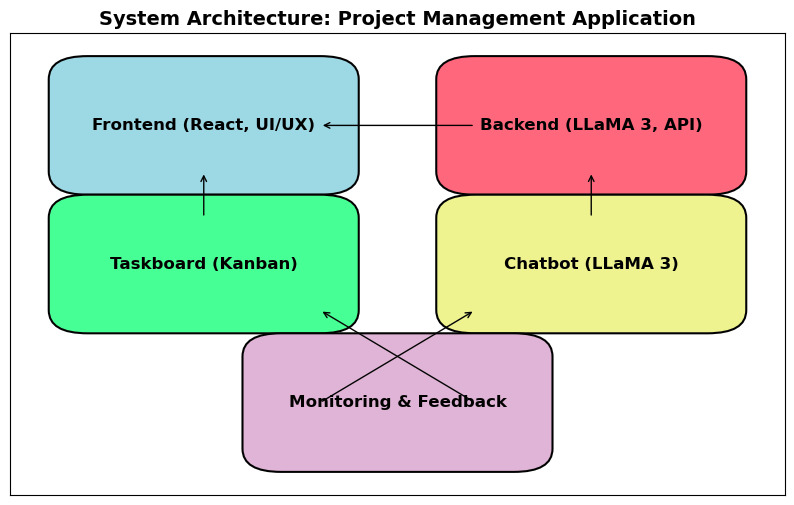
\includegraphics[scale=0.35]{images/grafica.jpg}
	
	
	\begin{thebibliography}{00}
		\bibitem{b1} 
	\end{thebibliography}
	
	
\end{document}